% !TeX root = ../main.tex

\chapter{基于3D高斯泼溅的水下三维重建}
3D 高斯泼溅(3DGS)\cite{3DGS} 已逐步取代神经辐射场(NeRF)\cite{nerf} 技术,成为场景重建领域的热门工具。
然而,目前尚缺乏针对水下环境的充分验证与应用研究,主要原因在于缺少专门用于此类任务的水下场景数据集支持。
此外,由于水下图像的退化效应(如光散射、色偏)及水流造成的动态扰动,水下场景重建需要超越静态场景重建的传统方法。
得益于神经网络的时空预测能力,3DGS 在动态场景的重建中也具备高质量的场景复现能力。
为此,本章提出了一种基于 3DGS 和 KAN \cite{kan}变形扩展的水下场景感知增强框架。
该框架旨在优化特定时刻下的静态场景表示,通过抑制运动干扰从而保留水下场景的基础静态特征。
同时,本章构建了一个专门面向水下场景重建的数据集,并在此数据集上对方法进行验证。
实验结果表明,与其他基准方法相比,本章提出的框架在准确性和鲁棒性方面具有显著优势。

\section{水下动态场景的3D高斯泼溅方法}
3D 高斯泼溅方法可以直接对场景信息进行显式表示,这为动态场景建模提供了一种灵活的解决方案。
其核心思想是通过变形每个时间点的 3D 高斯表示,寻找符合动态场景重建的最优变形方法。
目前,利用神经网络学习位置与时间信息的映射关系已成为主流方案。
在此基础上,本章基于时空信息编码与解码的4D高斯泼溅\cite{4DGS}框架为水下动态场景重建提供有效支持。
如图\ref{img:4dgs}所示,该框架通过时空结构编码器高效提取 3D 高斯的时空特征,并结合特征解码器实现高斯变形预测,从而提升水下动态场景重建的质量和效率。
\begin{figure}[htbp]
    \centering
    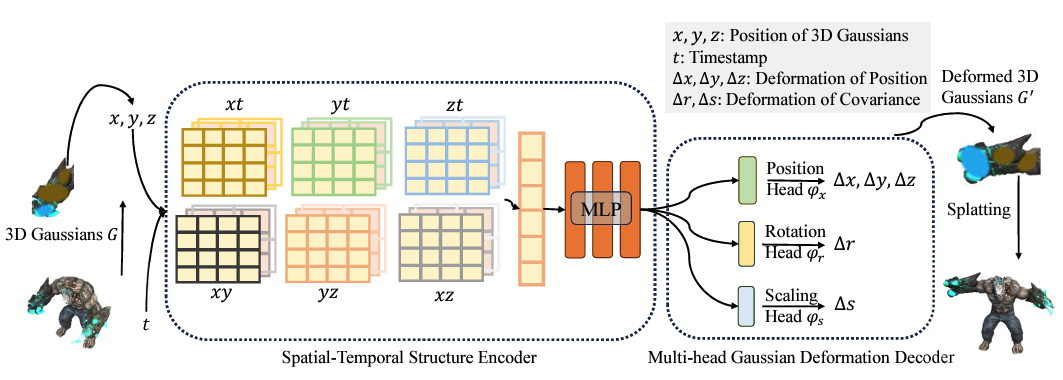
\includegraphics[width=0.8\textwidth]{figures/ch4/4dgs.jpg}
    \caption{基于 3D 高斯泼溅的水下动态场景重建框架}
    \label{img:4dgs}
\end{figure}

\subsection{3D高斯时空编码器}
动态场景中的相邻 3D 高斯通常具有显著的时空信息相似性。
为高效捕捉这些相似性特征,本章设计了一种时空结构编码器 $\mathcal{H}$,
该编码器由多个分辨率的 HexPlane 模块\cite{hex_plane} 和一个多层感知机(MLP)模块组成。
其主要目标是结合 3D 高斯的位置与时间信息,将其映射到低维特征空间,为后续多头解码器进行变形预测提供支持。

为了避免高维空间的维度灾难,本章的HexPlane模块采用了K-Planes\cite{k-planes}的方法将每个点的特征分解为它在空间中的特征和它在每个轴(XYZ)上关于时间的特征,从而优化内存占用并降低计算复杂度。
具体做法是将原始 4D 神经体素分解为 6 个独立的平面模块,这些模块能够有效表示一定区域内的 3D 高斯,并通过时间维度进一步捕捉高斯变形信息。
因此3D时空结构编码器$\mathcal{H}$包含6个多分辨率平面模块$R_l(i,j)$和一个小型MLP模块$\phi_d$,如公式\ref{eq:encoder_H}所示:
\begin{equation}
\label{eq:encoder_H}
\mathcal{H}(\mathcal{G}, t) = \{ R_l(i,j), \phi_d \ | \ (i,j) \in \{(x,y), (x,z), (y,z), (x,t), (y,t), (z,t)\}, l \in \{1, 2\} \}
\end{equation}

其中,$\mathcal{X} = (x, y, z)$表示3D高斯的中心位置,$l$表示上采样的尺度,
$R(i,j)$是每个体素平面模块,维度为$R(i,j) \in \mathbb{R}^{h \times l N_i \times l N_j}$,
其中$h$表示平面中单个网格特征的维度,$N_i,N_j$表示每个平面体素网格的基本分辨率。

为提取每个体素特征,需要在6个2D体素平面中对3D高斯体的信息进行编码,可以使用双线性插值的方法查询平面体素网格四个顶点的特征,计算公式为:
\begin{equation}
f_h = \bigcup_l \prod \text{interp}(R_l(i,j)), \quad (i,j) \in \{(x,y),(x,z),(y,z),(x,t),(y,t),(z,t)\}
\end{equation}

其中,$f_h \in \mathbb{R}^{h \times l}$表示神经体素的特征。
随后,MLP 模块 $\phi_d$ 融合所有特征以生成最终的编码表示:
\begin{equation}
f_d = \phi_d(f_h)
\end{equation}  

该编码过程不仅可以高效捕获动态场景中时空特征的变化,还为后续高斯变形计算奠定基础。

\subsection{基于KAN的特征解码器}
时空结构编码器生成的 3D 高斯特征随后被输入到多头高斯变形解码器 $\mathcal{D}$ 中,以计算每个 3D 高斯在不同时刻下的变形信息。
该解码器包含多个KAN模块,分别用于估计位置变形$\Delta \mathcal{X}$、旋转变形$\Delta r$和缩放变形$\Delta s$。
这些变形信息构成了变形后的 3D 高斯表示$\mathcal{G}^\prime=\{\mathcal{X}^\prime, s^\prime, r^\prime, \sigma, \mathcal{C} \}$。
KAN 模块通过学习神经元的最优激活方式,在保证解码准确性的同时减少了所需的神经元数量。
基于KAN的特征解码器通过自适应的方式预测形变量,最终的变形3D高斯可以表示为:
\begin{equation}
    \mathcal{G}^\prime = \{ \mathcal{X} + \Delta \mathcal{X}, r + \Delta r, s + \Delta s, \alpha + \Delta \alpha, \mathcal{C} + \Delta \mathcal{C} \}
\end{equation}

不同时刻下的3D高斯可以有效处理水下环境中的动态特征,生成精准的动态场景重建结果。

\section{水下静态三维场景自对抗训练}
\subsection{三阶段训练模优化}
在水下复杂环境中,由于水流带来的动态干扰,场景中的原始画面中的物体会发生一定晃动,使得无法完全在水下进行静态的场景工作,基于动态场景重建的方法来对水下环境进行保留动态效果的新视图生成,可以一定程度上可以到的高质量且逼真的渲染结果。但是在利用单目相机拍摄的水下动态场景建模时,会出现某些时刻的场景重建异常的现象,这主要是由于单目相机在该时刻附近3D 高斯的建模缺乏足够多的视角数据,导致变形预测结果的错误。

假定水下重建场景中的各个对象的位置相对固定,可以认为水流带来的扰动会让水下对象呈一种周期往复的抖动,在这种条件下,本文提出了运动干扰视角过滤方法,在前期动态重建的基础上,提取水下对象变化中3D 高斯高度相似的时刻,从而实现对某一相对固定对象的静态重建,过滤出不能完整渲染不同视角的时刻。

如图所示,首先用3DGS的方法进行小迭代次数的第一阶段的粗训练,得到3D 高斯的初始化信息,再结合KAN进行动态阶段场景的重建训练,此过程中可以基本完成水下动态场景的重建效果,但可能某些时刻下场景的渲染质量较差,接下来进行第三阶段的静态阶段训练,通过统计动态场景重建的不同时刻下的场景信息,从中剔除重复度低的数据,保留大多数相似的高频数据,从而在最后的渲染过程中达到去除水流扰动的效果。

\subsection{运动时空过滤模块}
为了保证运动时空过滤模块可以过滤出不需要的训练数据,同时降低显存占用,要对全部的不同时刻下的3D 高斯进行两次遍历,第一次遍历通过累计求和的方式得到每个3D 高斯的平均位置作为过滤的基准,再经过第二次遍历在所有训练数据中筛选出与平均位置相似的数据并记录保存这些时刻$t_{static}$。如图所示,时空过滤模块从不同时刻的高斯中筛选出有效数据并进行第三阶段的训练。

需要指出的是,在最后静态场景的训练阶段,会依旧保留动态重建的变形机制,带有时序信息的训练可以一定程度减少由于时空过滤错误带来的负面影响,提升对过滤模块的宽容度。

\subsection{损失函数设计}
与其他重建方法类似\cite{3DGS},本文采用L1颜色损失(L1 Color Loss)来监督训练过程,确保生成的3D高斯在颜色方面与目标场景的实际颜色保持一致。此外,还引入了基于网格的全变差损失(Total Variation Loss,$\mathcal{L}_{tv}$)\cite{hex_plane}\cite{k-planes},以减少噪声并提高重建结果的平滑性。全变差损失有助于控制空间中不连续点的变化,从而提高模型在重建过程中的稳定性,特别是在处理高频细节和复杂动态场景时。

L1颜色损失用于衡量生成的场景颜色与真实场景颜色之间的绝对误差,计算公式为:
$$
\mathcal{L}_{color} = \sum_{i} \left\| \hat{C}_i - C_i \right\|_1
$$

其中,$\hat{C}_i$是模型生成的第$i$个像素的颜色值,$C_i$是对应的真实颜色值。

全变差损失则是对生成的3D高斯网格中像素值变化的度量,目标是减少不必要的细节和噪声,保持图像的平滑性。其计算公式为:
$$
\mathcal{L}_{tv} = \sum_{i,j} \left\| \nabla \mathcal{G}(i,j) \right\|_2
$$

其中,$\nabla \mathcal{G}(i,j)$表示网格中位置$(i,j)$的梯度,衡量的是相邻体素之间的变化。这个损失项在训练过程中有助于避免模型过度拟合细节,从而提高重建的鲁棒性。

最终,训练的总损失由颜色损失和全变差损失加权组合得到:
$$
\mathcal{L}_{total} = \mathcal{L}_{color} + \lambda_{tv} \cdot \mathcal{L}_{tv}
$$

其中,$\lambda_{tv}$是全变差损失的权重系数,用于平衡颜色损失和平滑性损失之间的影响。通过最小化该总损失,模型能够在重建动态场景的同时保持高精度的颜色一致性,并避免过多的噪声。

\section{实验结果}
\subsection{水下重建数据集制作}
为了验证水下重建工作的有效性,本文制作了第一个用于水下重建工作的数据集 3DUW,通过单目相机搜集了几种水下场景的在不同时刻的多角度图片,同时在拍摄时人为制造一些水流的干扰,使物体在水下呈现自然的摆动。最后用运动结构算法(SFM)\cite{sfm1}\cite{sfm2}来对采集的数据进行预处理,得到不同图像的相机位姿信息以及初始点云。

\subsection{实验设置}
本文对比了两组数据集:自建的3DUW数据集和公开的动态场景重建数据集D-NeRF\cite{dnerf}。D-NeRF是一个合成数据集,每个场景包含50到200帧数据,且每一帧的相机位姿是随机生成的。
时空编码器与解码器主要使用PyTorch框架\cite{pytorch}进行实现。所有测试均在单个RTX 3060 GPU上进行。3DGS粗训练阶段、动态训练阶段以及静态训练阶段的迭代次数分别设置为3000、20000和10000次。

\subsection{定量评价}
为评估重建结果,我们采用了多种评价指标,包括峰值信噪比(PSNR)、感知质量指标LPIPS\cite{lpips}、结构相似性指数(SSIM)\cite{ssim}及其扩展指标(如结构不相似指数DSSIM、多尺度结构相似性指数MS-SSIM)、帧率(FPS)和训练时间等,用于衡量新视角合成的质量。此外,我们还对该领域的多个先进方法进行了基准测试,
如??????????等。值得注意的是,由于本文采用了运动时空过滤模块,因此在动态训练阶段之后,需要对测试数据集进行类似的过滤过程。在D-NeRF数据集中,这一过程可以理解为保留全局空间点云运动中最频繁出现的位置,作为静态场景的选择标准。对于3DUW数据集,视角过滤模块能够选择由于水流扰动引起的物体中心位置,并将其纳入静态阶段训练数据中。D-NeRF数据集由于缺乏3DUW数据集中动态运动特性,因此在视角过滤后得到的样本数量较少。具体的过滤样本数量如表所示。

\subsection{定性评价}
4DGS能够生成高质量的动态新视角,但在某些时刻,某些视角的渲染效果不佳,尤其是动态帧之间的运动过渡不够平滑,并且它们之间的间隔过大。本文分析认为这些时刻的某些视角数据属于相对孤立的数据点,常常导致某些视角出现崩溃现象。这些孤立数据点会对其他正常训练数据的视觉细节造成负面影响。

针对消除水下扰动的影响,本文提出的方法能够有效地过滤掉由水流扰动引起的孤立数据,同时保留相对未受干扰的原始场景并进行重建。如图所示,在3DUW数据集中,我们的过滤结果能够准确地提取出水下物体的中心摆动位置。

\subsection{结果讨论}
KAN:KAN在形变解码器中扮演了关键角色,负责对不同3D高斯的时空特征进行多头解码。与MLP相比,尽管KAN会增加训练时间,但它显著提升了最终渲染结果的质量。如表所示,实验结果表明,去除KAN会减少训练时间,但渲染质量有所下降。

运动时空过滤模块:基于水下原始捕获的数据中存在相对孤立的场景信息,会对结果产生负面影响。时空过滤模块在水下动态场景的训练结束时进行数据筛选。如图所示,时空过滤模块能够有效地过滤掉这些孤立数据,从而进一步提高渲染细节和增强渲染质量。如表所示,经过视角过滤后保留下来的数据进行进一步训练,能够改善水下重建结构,并消除由水下运动干扰引起的负面影响。

局限性:本章提出的方法能够成功渲染水下数据集3DUW中水下运动的静态中心场景,但仍然存在一些困难和挑战需要解决。首先,为了确保视角过滤能够选择足够的训练数据,需要使用间隔尽可能小的动态帧,这样物体的静态中心才能拥有足够的相机位姿。其次,由于视角过滤规则的局限性,目前的方法无法同时选择多个水下物体的运动中心,这使得本章的方法更适用于由单一水下物体引起的扰动重建。